\documentclass[tikz,border=10pt]{standalone}
\usetikzlibrary{angles,quotes,calc}
\begin{document}
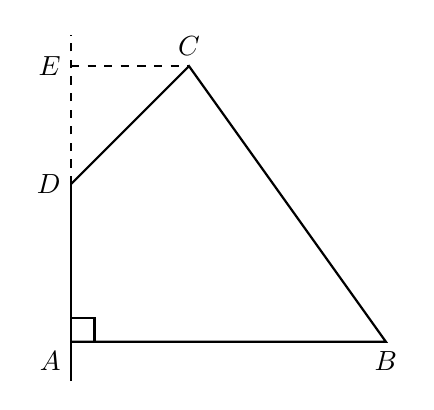
\begin{tikzpicture}[>=stealth, thick]
    % 1. 定义坐标 (按比例预设)    
\coordinate (A) at (0,0);    
\coordinate (B) at (4,0);    
\coordinate (D) at (0,2);    
\coordinate (C) at (1.5,3.5);    
\coordinate (E) at (0,3.5);     
\coordinate (P) at (0,3.9);
    % 2. 绘制主体图形 (多边形)    
\draw (A) -- (B) -- (C) -- (D);    
\draw (A) -- (D); % 垂直实线部分
    % 3. 绘制辅助线 (虚线)    
\draw (0,-0.5) -- (D); % 延长参考线    
\draw[dashed] (D) -- (P);       % 延长参考线    
\draw[dashed] (E) -- (C);       % 水平辅助线
    % 4. 标注直角符号    
\draw (0.3,0) -- (0.3,0.3) -- (0,0.3);
    % 5. 标注点位    
\node[below left] at (A) {$A$};    
\node[below] at (B) {$B$};    
\node[left] at (D) {$D$};    
\node[above] at (C) {$C$};    
\node[left] at (E) {$E$};
\end{tikzpicture}
\end{document}